%%%%%%%%%%%%%%%%%%%%%%%%%%%%%%%%%%%%%%%%%%%%%%%%%%%%%%%%%%%%%%%%%%%%%%%%%%%%%%%%
\section{Message Authentication}
\label{sec:msgauth}

A message authentication scheme $\MA = (\kg,\mtag,\ver)$ is a triple of
algorithms. Key generation is randomized and outputs a key. Message
authentication $\mtag$ takes as input a key and message and outputs a tag.
Verification takes as input a key, a message, and a tag, and outputs a bit. 

A message authentication scheme is correct if for all keys $K$ from $\kg$ and messages $M\in \msgset$, 
\bnm
\Prob{\ver(K,M,\mtag(K,M))=1}=1\;.
\enm

One specific variant of message authentication schemes is a $\MACscheme$, a Message Authentication Code. For a $\MAC$, the $\mtag$ function is deterministic, so 
\bnm
\ver(K,M,T)=(\mtag(K,M)=T)\;,
\enm
where the probability is over any random coins in $\mtag$.
\begin{figure}[t]
	\centering
	\hfpagesss{.2}{.25}{.25}{
		\underline{$\UFCMA_\MA^\advA$}\\[1pt]
		$K \getsr \kg$\\
		$(M^*,T^*) \getsr \advA^{\TagOracle}$\\
		If $M^* \in \msgset$ then\\
		\myInd Ret $\false$\\
		Ret $\ver(K,M^*,T^*)$\medskip
		
		\underline{$\TagOracle(M)$}\\
		$\msgset \gets \msgset \cup \{M\}$\\
		Ret $\mtag(K,M)$
	}
	{
	\underline{$\SUFCMA_\MA^\advA$}\\[1pt]
	$K \getsr \kg$\\
	$\win\gets\false$\\
	$(M^*,T^*) \getsr \advA^{\TagOracle,\VerOracle}$\\
	Ret $\win$\medskip
	}{
	\underline{$\TagOracle(M)$}\\
	$T \gets \mtag(K,M)$\\
	$\pairset \gets \pairset \cup \{(M,T)\}$\\
	Ret $T$\medskip 
	
	\underline{$\VerOracle(M,T)$}\\
	If $(M,T) \in \pairset$ then \\
	\myInd Ret $\bot$\\
	$b \gets \ver(K,M,T)$\\
	If $b = 1$ then $\win\gets\true$\\
	Ret $b$
	}	
	\caption{Games for $\UFCMA$ and $\SUFCMA$ security of message authentication schemes.}
	\label{fig:game-ufcma}
\end{figure}

For security of a message authentication scheme, we ask that no computationally efficient adversary is able to forge a tag for a message, even in a chosen message attack. This notion is formalized in the $\UFCMA_\MA$ (Unforgeability under Chosen Message Attack) game in Figure~\ref{fig:game-ufcma}. An adversary $\advA$ has access to a $\TagOracle$ oracle, and its goal is to return a pair $(M^*,T^*)$ such that it never received the tag of $M^*$ through the $\TagOracle$ oracle, and $T^*$ is a valid tag of $M^*$. 

We say that the advantage of the $\UFCMA_\MA$ adversary $\advA$ is 
\bnm
  \AdvUFCMA{\MA}{\advA} = \Prob{\UFCMA_\MA^\advA\Rightarrow 1}.
\enm

We can also ask for a stronger notion of unforgeability, where the adversary is able to make more than just one attempt at forging a tag. This is formalized in the $\SUFCMA_\MA$ game in Figure~\ref{fig:game-ufcma}. In this game, the adversary gets access to a $\VerOracle$ oracle as well as a $\TagOracle$ oracle, and it wins if it makes a query to $\VerOracle$ with a valid message and tag pair. Another difference with $\SUFCMA_\MA$ is that an adversary can win with a message that was queried to $\TagOracle$, as long as the tag it gives is different. We define the advantage of a $\SUFCMA_\MA$ adversary $\advA$ as 
\bnm
  \AdvSUFCMA{\MA}{\advA} = \Prob{\SUFCMA_\MA^\advA\Rightarrow 1} 
\enm

If a message authentication scheme $\MA$ is $\SUFCMA_\MA$ secure, then it is also $\UFCMA_\MA$ secure, as stated in Theorem~\ref{thm:sufcma-ufcma}. The proof of Theorem~\ref{thm:sufcma-ufcma} is left to the reader in~\ref{exercise:sufcma-ufcma}.
\begin{theorem}
	\label{thm:sufcma-ufcma}
Let $\MA = (\kg,\mtag,\ver)$ be a message authentication scheme. Then for any $\UFCMA_\MA$-adversary $\advA$ making $q$ queries, we give a $\SUFCMA_\MA$ adversary $\advB$ making $q$ queries such that
\bnm
	\AdvUFCMA{\MA}{\advA} \le \AdvSUFCMA{\MA}{\advB} \;.
\enm
\end{theorem}

In general, it is not true that $\UFCMA_\MA$ security of a message authentication scheme $\MA$ implies $\SUFCMA_\MA$ security. However, if $\MA$ is a $\MAC$, then $\UFCMA_\MA$ security is equivalent to $\SUFCMA_\MA$. This proof is left to~\ref{exercise:mac-sufcma-ufcma}.
We can construct a $\UFCMA_\MA$ secure MAC using a good PRF. The associated MAC for a PRF $F$ is:
\bnm
\mtag(K,M)=F(K,M)\myInd\myInd \ver(K,M,T)=(F(K,M)=T)
\enm

\begin{theorem}
Let $F\Colon\bits^k\times\msgspace\rightarrow\bits^n$. Then for any
$\UFCMA_F$-adversary $\advA$ making $q$ queries, we give a $\PRF_F$-adversary $\advB$ such that
\bnm
  \AdvUFCMA{F}{\advA} \le \AdvPRF{F}{\advB} + \frac{1}{2^n} \;.
\enm
Adversary $\advB$ runs in time that of $\advA$ and makes $q+1$ queries.
\label{thm:prf-ufcma}
\end{theorem}

\begin{figure}
\centering
\fpage{.2}{
	\underline{$\G0$}\\[1pt]
	$K \getsr \bits^k$\\
	$(M^*,T^*) \getsr \advA^{\TagOracle}$\\
	If $M^* \in \msgset$ then\\
	\myInd Ret $\false$\\
	Ret $F(K,M^*)=T^*$\medskip

	\underline{$\TagOracle(M)$}\\
	$\msgset \gets \msgset \cup \{M\}$\\
	Ret $F(K,M)$
}
\fpage{.2}{
	\underline{$\G1$}\\[1pt]
	$(M^*,T^*) \getsr \advA^{\TagOracle}$\\
	If $M^* \in \msgset$ then\\
	\myInd Ret $\false$\\
	Ret $\Horacle(M^*)=T^*$\medskip
	
	\underline{$\TagOracle(M)$}\\
	$\msgset \gets \msgset \cup \{M\}$\\
	Ret $\Horacle(M)$\medskip
	
	\underline{$\Horacle(M)$}\\[1pt]
	If $T[M] = \bot$ then \\
	\myInd $T[M]\getsr \bits^n$\\
	Ret $T[M]$
}
\fpage{.22}{
	\underline{$\advB^{\Fn}$}\\[1pt]
	$(M^*,T^*) \getsr \advA^{\TagSim}$\\
	If $\Fn(M^*)=T^*$ then Ret 1\\
	Else Ret 0\medskip
	
	\underline{$\TagSim(M)$}\\[1pt]
	Ret $\Fn(M)$
}
\caption{Games and adversary for proof of Theorem~\ref{thm:prf-ufcma}.}
\label{fig:games-prf-ufcma}
\end{figure}

\begin{proof}
	We will refer to the games and adversary in Figure~\ref{fig:games-prf-ufcma}. Game $\G0$ is the same as the game $\UFCMA_F$.
	\bnm
	\Prob{\G0}=\Prob{\UFCMA_F^\advA\outputs 1}=\AdvUFCMA{F}{\advA}
	\enm
	In Game $\G1$, the tag of a message is chosen uniformly at random from $\bits^n$, the output space of $F$. Therefore, even if $\advA$ returns some $M^*\notin \msgset$, the probability that $T^*$ is the correct tag is the chance that $T^*$ is the string that was sampled randomly.
	\bnm
	\Prob{\G1}\leq \frac{1}{2^n}
	\enm
	The advantage of $\UFCMA_F$-adversary $\advA$ is bounded as
	\begin{align*}
	\Prob{\G0}=(\Prob{\G0}-\Prob{\G1}) + \Prob{\G1}\\
	\AdvUFCMA{F}{\advA}\leq (\Prob{\G0}-\Prob{\G1}) + \frac{1}{2^n}\;.
	\end{align*}
	Next, we claim that the advantage of $\PRF_F$-adversary $\advB$ is
	\bnm
	\AdvPRF{F}{\advB} =\Prob{\PRF1_F^\advB\Rightarrow 1}-\Prob{\PRF0_F^\advB\Rightarrow 1} = \Prob{\G0}-\Prob{\G1}\;.
	\enm
	First, if the output of $\Fn$ is real, then $\advB$ outputs 1 if and only if $\advA$ wins in $\G0$, so
	\bnm
	\Prob{\PRF1_F^\advB\Rightarrow 1}=\Prob{\G0}\;.
	\enm
	If the output of $\Fn$ is random, $\advB$ outputs 1 if and only if $\advA$ wins in $\G1$, so 
	\bnm
	\Prob{\PRF0_F^\advB\Rightarrow 1}=\Prob{\G1}\;.
	\enm
	Therefore, we can say that 
	\bnm
	\AdvUFCMA{F}{\advA} \le \AdvPRF{F}{\advB} + \frac{1}{2^n} \;.
	\enm
\end{proof}

To actually build a variable input length PRF that can be used as a MAC, we can start with the CBC construction we have seen before (Fig~\ref{fig:cbc-mac}).

\begin{figure}
\centering
        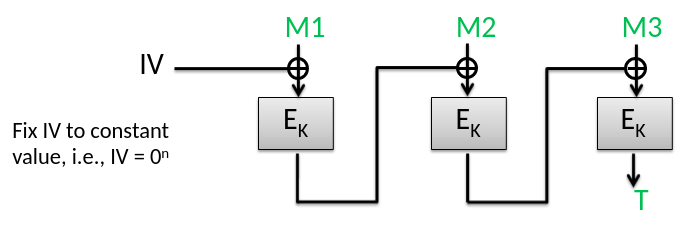
\includegraphics[width=0.5\textwidth]{notes/cbc-mac.png}
    \caption{CBC-MAC construction.}
    \label{fig:cbc-mac}
\end{figure}

To modify the construction to be deterministic, we can set the IV to be $0^n$. The output will be the final block of the ciphertext. However, the CBC-MAC construction doesn't satisfy $\UFCMA$ security. The adversary below gets advantage 
\bnm
\AdvUFCMA{\CBC\text{-}\MAC}{\advA}=1\;.
\enm
\begin{figure}[h]
	\centering
\fpage{.20}{
	\underline{$\advA^{\Tag}$}\\[1pt]
	$T_1 \gets \TagOracle(0^n)$\\
	$M = 0^n\concat T_1$\\
	Ret $(M,T_1)$
}
\end{figure}

However, we give a modified construction, Encrypted CBC-MAC (ECBC-MAC), that uses the same block cipher, $\E$, with a different key $K_2$ to encrypt the final output of the CBC-MAC. \scribenote{give either pseudocode or diagram of the construction.} We will prove that for any function $H$ that is an  $\epsilon$-almost universal (AU) hash function, the ECBC-MAC construction is a good variable input length $\PRF$. 

First, we define what it means to be an $\epsilon$-almost universal (AU) hash function.

A keyed function $H\Colon\bits^k\times\msgspace\rightarrow\bits^n$ is
an $\epsilon$-almost universal (AU) hash function  if for all $M,M'\in\msgspace$, $M \ne M'$
\bnm
  \Prob{H_K(M) = H_K(M')} \le \epsilon
\enm
where the probability is over random choice of $K$.

A computational almost universal (\cAU) hash function is a function for which all polynomial-time bounded $\cAU_H$ adversaries $\advA$ have small $\cAU_H$ advantage.
\begin{figure}[h]
\centering
\fpage{.20}{
\underline{$\cAU_H^\advA$}\\[1pt]
$M,M' \getsr \advA$\\
$K \getsr \bits^k$\\
If $M = M'$ then Ret $\false$\\
Ret $H_K(M) = H_K(M')$
}
\end{figure}

We define the advantage of a $\cAU_H$ adversary $\advA$ as
\bnm
  \AdvcAU{H}{\advA} = \Prob{\cAU^\advA_H\Rightarrow\true}\;.
\enm

\begin{figure}[h]
	\centering
	\fpage{.20}{
		\underline{$V(K,M)$}\\[1pt]
		$K_1,K_2\gets K$\\
		Ret $F(K_1, H(K_2,M))$\\
	}
\end{figure}
\begin{theorem} \label{thm:cau-vil-prf}
Let $F\Colon\bits^{k_1}\times \bits^n\rightarrow \bits^n$ be a fixed input length PRF, and let $H\Colon \bits^{k_2}\times \msgspace\rightarrow \bits^n$ be a $\cAU$ hash function. Let $V\Colon \bits^{k_1+k_2}\times \msgspace \rightarrow \bits^n$ be the variable input length PRF constructed using $F$ and $H$ as described above. Then, for any $\PRF_V$ adversary $\advA$ making $q$ queries, we can construct a $\cAU_H$ adversary $\advB$ and $\PRF_F$ adversary $\advC$ such that 
\bnm
	\AdvPRF{V}{\advA} \le \AdvcAU{H}{\advB} + \AdvPRF{F}{\advC}\;.
\enm
\scribenote{Above is a tentative theorem statement. Will fix once I write a proof.}
\end{theorem}

We show that if $E$ is a good PRF, then the CBC-MAC construction is computational almost universal.
\begin{theorem}
Let $E\Colon\bits^k\times\bits^n\rightarrow\bits^n$ and $H$ be the CBC-MAC. 
Then for any $\cAU_H$-adversary $\advA$ outputting messages of length at most
$\sigma$ blocks, for $\sigma\leq 2^n/4$, we give a $\PRF_E$-adversary $\advB$
such that
\bnm
  \AdvcAU{H}{\advA} \le \AdvPRF{E}{\advB} + \frac{\sigma^2}{2^n} \;.
\enm
Adversary $\advB$ runs in time that of $\advA$ and makes at most $2\sigma$
queries.
\label{thm:cau-cbcmac}
\end{theorem}
\begin{figure}
\centering
\fpage{.2}{
	\underline{$\G0$}\\[1pt]
	$M,M' \getsr \advA$\\
	$K \getsr \bits^k$\\
	If $M = M'$ then Ret $\false$\\
	$T \gets 0^n\semi T'\gets 0^n$ \\
	For $i=1$ to $m$ do \\
	\myInd $T\gets H_K(T\xor M[i])$\\
	For $j=1$ to $m'$ do \\
	\myInd $T'\gets H_K(T'\xor M'[j])$\\
	If $T=T'$ then Ret 1\\
	Ret $T=T'$
}
\fpage{.2}{
	\underline{$\G1$}\\[1pt]
	$M,M' \getsr \advA$\\
	If $M = M'$ then Ret $\false$\\
	$T \gets 0^n\semi T'\gets 0^n$ \\
	For $i=1$ to $m$ do \\
	\myInd $T\gets \Horacle(T\xor M[i])$\\
	For $j=1$ to $m'$ do \\
	\myInd $T'\gets \Horacle(T'\xor M'[j])$\\
	Ret $T=T'$\medskip
	
	\underline{$\Horacle(M)$}\\[1pt]
	If $T[M] = \bot$ then \\
	\myInd $T[M]\getsr \bits^n$\\
	Ret $T[M]$
}
\fpage{.22}{
	\underline{$\advB^{\Fn}$}\\[1pt]
	$M,M' \getsr \advA$\\
	If $M=M'$ then Ret 0 \\
	$T \gets 0^n\semi T'\gets 0^n$ \\
	For $i=1$ to $m$ do \\
	\myInd $T\gets \Fn(T\xor M[i])$\\
	For $j=1$ to $m'$ do \\
	\myInd $T'\gets \Fn(T'\xor M'[j])$\\
	If $T=T'$ then Ret 1\\
	Else Ret 0
}
\caption{Games and adversary for proof of Theorem~\ref{thm:cau-cbcmac}.}
\label{fig:games-cau-cbcmac}
\end{figure}

\begin{proof}
	We refer to the games and adversary in Figure~\ref{fig:games-cau-cbcmac}. Let $m$ and $m'$ respectively be the number of blocks in messages $M$ and $M'$ outputted by the $\cAU$ adversary $\advA$. 
	
	The games just explicitly describes the CBC-MAC construction within the $\cAU$ game, so 
	\bnm
	\AdvcAU{H}{\advA}=\Prob{\G0}\;.
	\enm
	Adversary $\advA$ wins in $\G1$ if there is a collision in either the inputs or the outputs of the random oracle that results in $T$ being equal to $T'$. A detailed analysis of this can be found in~\cite{black2000cbc}, and it turns out that we can bound this probability by 
	\bnm
	\Prob{\G1}\leq \frac{\sigma^2}{2^n}\;.
	\enm
	By examination, we can see that 
	\bnm
	\Prob{\PRF1_F^\advB\Rightarrow 1}=\Prob{\G0}
	\enm
	and
	\bnm
	\Prob{\PRF0_F^\advB\Rightarrow 1}=\Prob{\G1}\;.
	\enm
	Combining these, we see that 
	\begin{align*}
	\Prob{\G0}&=(\Prob{\G0}-\Prob{\G1}) + \Prob{\G1}\\
	\AdvcAU{H}{\advA}&\leq \AdvPRF{E}{\advB} + \frac{\sigma^2}{2^n}
	\end{align*}
\end{proof}

\section*{Exercises}
\begin{enumerate}[label=\textbf{Exercise \thesection.\arabic*}, wide=0pt]
	\item Prove Theorem~\ref{thm:sufcma-ufcma}. \label{exercise:sufcma-ufcma}
	\item Show that if a message authentication scheme $\MA$ is a $\MAC$, then $\UFCMA_\MA$ security is equivalent to $\SUFCMA_\MA$ security. \label{exercise:mac-sufcma-ufcma}
	\item Prove Theorem~\ref{thm:cau-vil-prf}.
\end{enumerate}